%Assignment 2 
%Vikas Kurapati
%130010058
\documentclass[11pt, a4paper]{article}
\usepackage[affil-it]{authblk} 
\usepackage{etoolbox}
\usepackage{lmodern}
\usepackage{titlesec}
\usepackage{float}

\makeatletter
\patchcmd{\@maketitle}{\LARGE \@title}{\fontsize{20}{19.2}\selectfont\@title}{}{}
\makeatother

\renewcommand\Authfont{\fontsize{16}{14.4}\selectfont}
\renewcommand\Affilfont{\fontsize{12}{10.8}\itshape}

\title{\textbf{End Semester:AE 647}} 
\author{Vikas Kurapati - 130010058}
\usepackage{graphicx}
\begin{document}
\maketitle
\newpage
\section{Question1}
The following formulae were used to calculate the required values:
\begin{equation}
 \lambda_D = \sqrt{\frac{\epsilon_0 kT_e}{n_eq_e^2}}
\end{equation}
\begin{equation}
 \rho_c = \frac{mv_\bot}{qB}
\end{equation}
\begin{equation}
 \lambda_{mfp} = \frac{36\pi \epsilon_0 kT_e}{ne^4}
\end{equation}
\begin{equation}
 \omega_{pe} = \sqrt{\frac{ne^2}{m_e \epsilon_0}}
\end{equation}
\begin{equation}
 \lambda_D = \frac{|q| B}{m}
\end{equation}
\begin{equation}
 \beta = \frac{2*\nu_0 nkT}{B^2}
\end{equation}

The following values have been obtained for $\frac{\lambda_d}{\rho_c}$as shown in plot.
\begin{figure}[H]
 \centering
 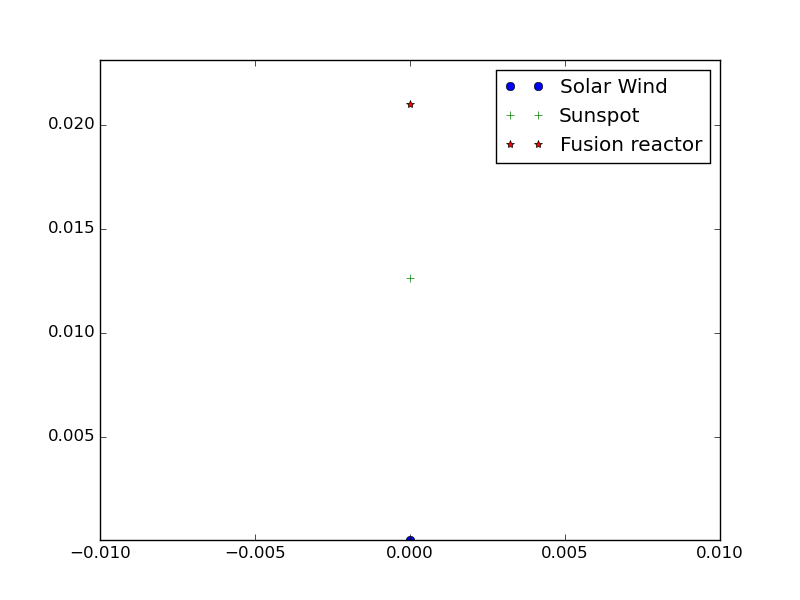
\includegraphics[width = \textwidth]{q1_0.png}
\end{figure}
The following values have been obtained for $\frac{\lambda_d}{\lambda_{mfp}}$as shown in plot.
\begin{figure}[H]
 \centering
 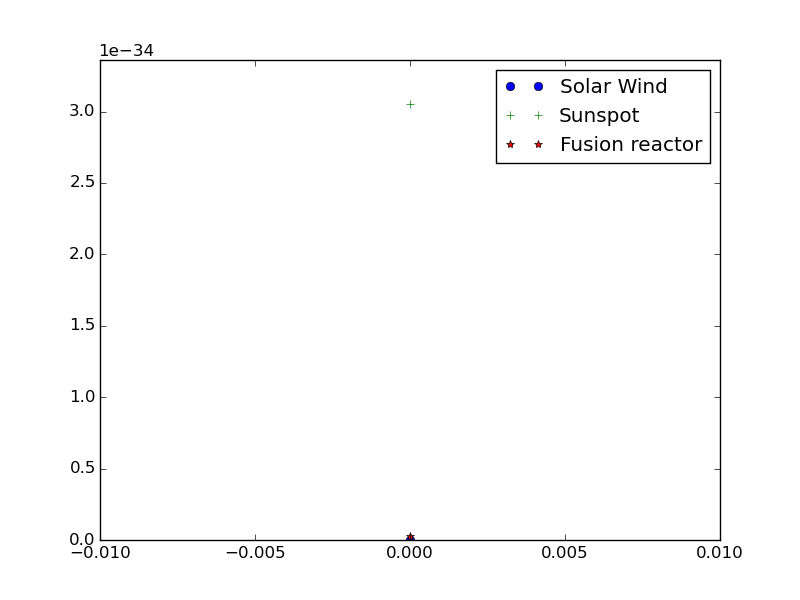
\includegraphics[width = \textwidth]{q1_1.png}
\end{figure}
The following values have been obtained for $n\lambda_D^3$as shown in plot.
\begin{figure}[H]
 \centering
 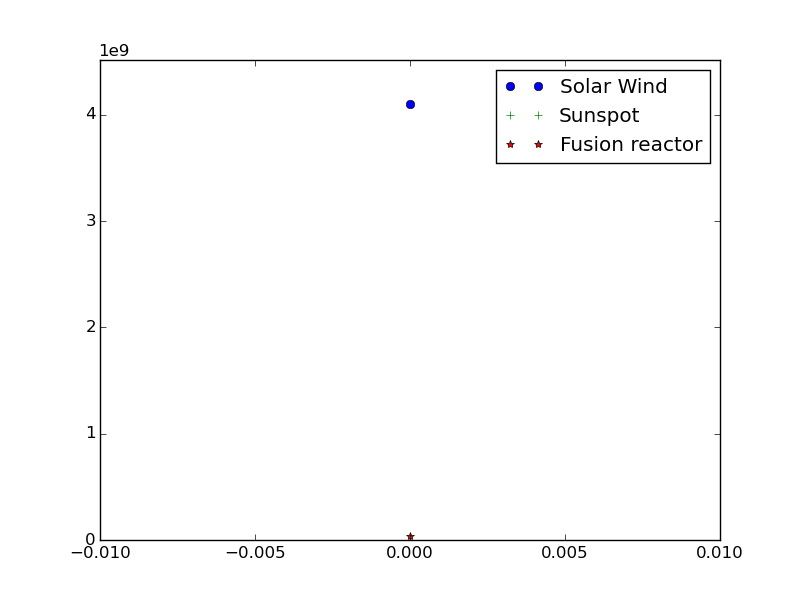
\includegraphics[width = \textwidth]{q1_2.png}
\end{figure}
The following values have been obtained for $\frac{\omega_{pe}}{\omega_{ce}}$as shown in plot.
\begin{figure}[H]
 \centering
 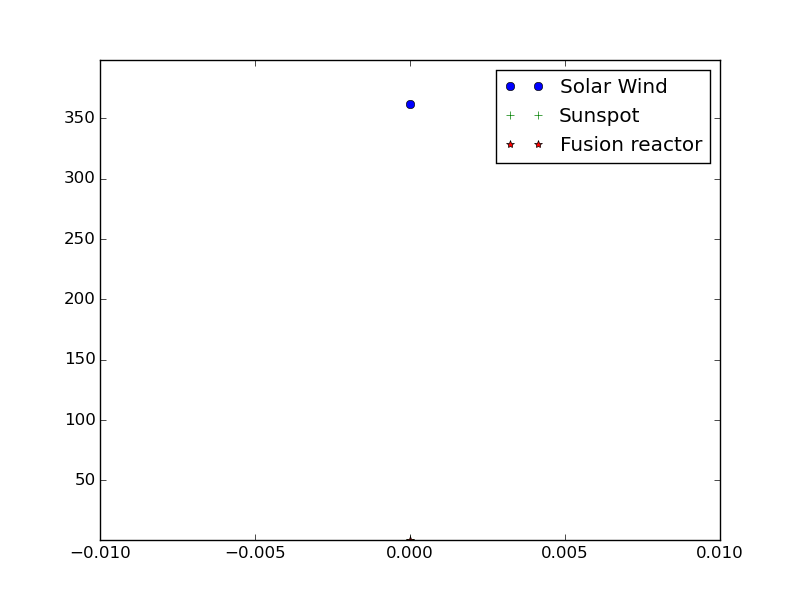
\includegraphics[width = \textwidth]{q1_3.png}
\end{figure}
The following values have been obtained for $\beta$as shown in plot.
\begin{figure}[H]
 \centering
 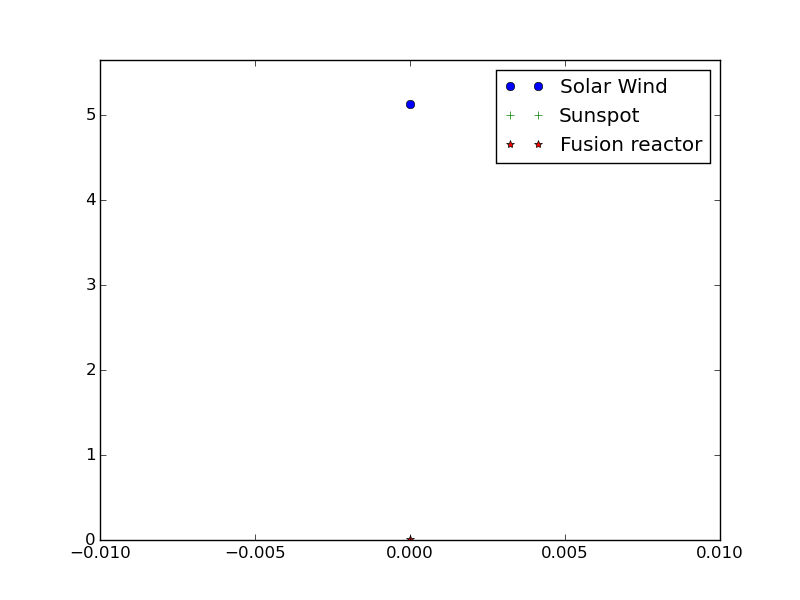
\includegraphics[width = \textwidth]{q1_4.png}
\end{figure}
Also the values of the required values are printed as matrices in the console for comparision as the plots are not very clear due to the small values of some of the parameters.

\section{Question2}
The following plot shows the variation of magnetic moment with time for zero Electric field case. It can be seen that the variation is low when compared to the original value by examining the value on the y-axis.
\begin{figure}[H]
 \centering
 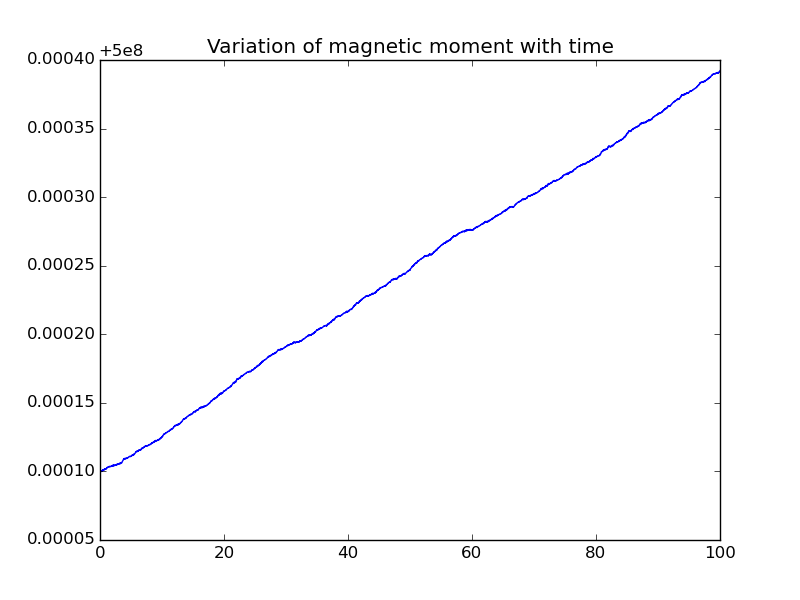
\includegraphics[width = \textwidth]{q2a1.png}
\end{figure}
The following plot shows the variation of magnetic moment with time for zero Electric field case. It can be seen that the variation is low when compared to the original value by examining the value on the y-axis.
\begin{figure}[H]
 \centering
 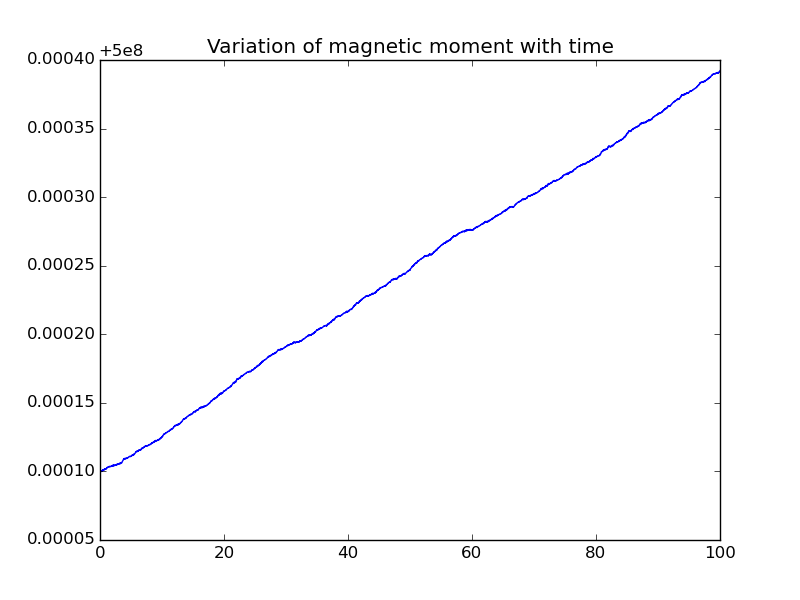
\includegraphics[width = \textwidth]{q2a2.png}
\end{figure}
Under the influence of a fluctuating Electric field, it can be seen from the plots that the analytical solution which uses drift velocity to compute the path as the concept of drift velocity is valid only for constant or slowly varying  electric fields.
\begin{figure}[H]
 \centering
 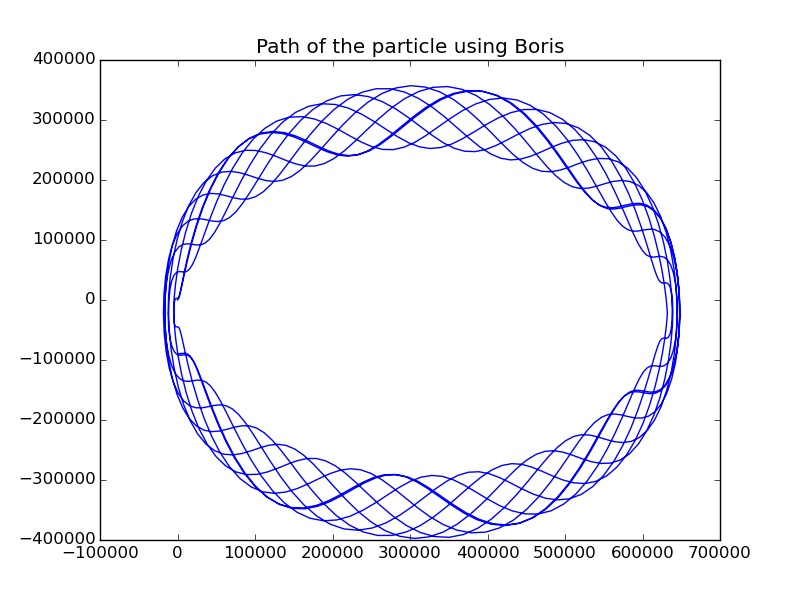
\includegraphics[width = \textwidth]{q2b_path.png}
\end{figure}
\begin{figure}[H]
 \centering
 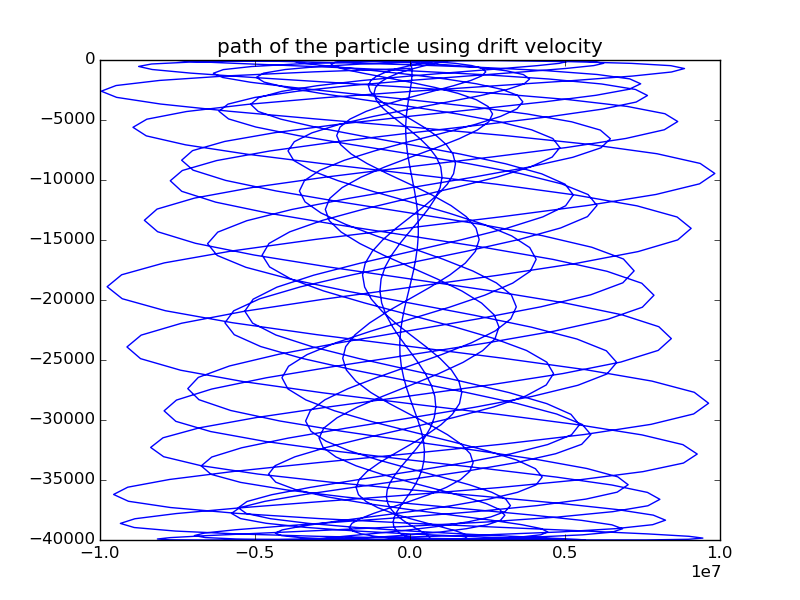
\includegraphics[width = \textwidth]{q2b_exact.png}
\end{figure}
The following plot shows the variation of magnitude of velocity with time. It can be seen the velocity fluctuates rapidly as a result of fluctuating electric field.
\begin{figure}[H]
 \centering
 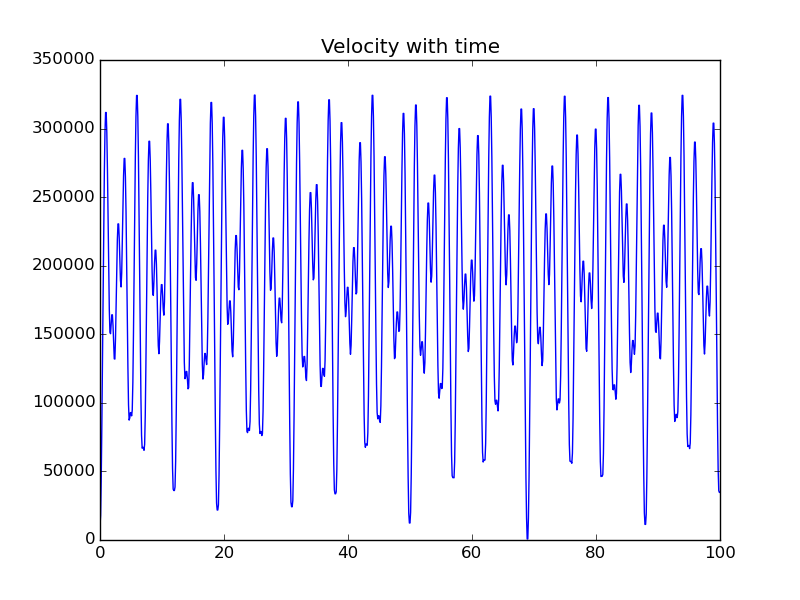
\includegraphics[width = \textwidth]{q2b_vel.png}
\end{figure}
Due to the high fluctuating nature of the electric field, it is expected that the electrical conductivity of the plasma is fluctuating about the initial value depending on the initial velocity almost sinusoidally. \\

The following plot shows the path of the particle under sunspot condition with initial conditions which can be changed in code.(Please refer code for initial conditions).
\begin{figure}[H]
 \centering
 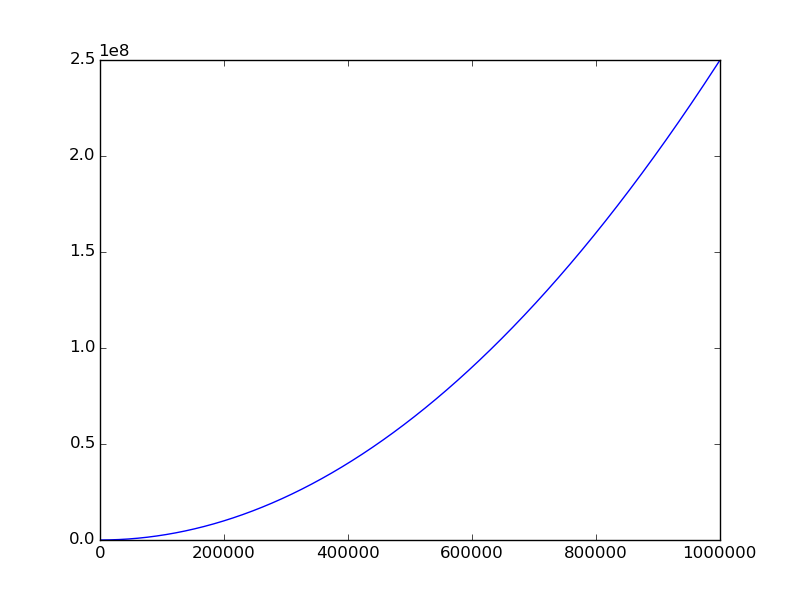
\includegraphics[width = \textwidth]{q2c_path.png}
\end{figure}
The following plot shows the velocity of the particle with time.
\begin{figure}[H]
\centering
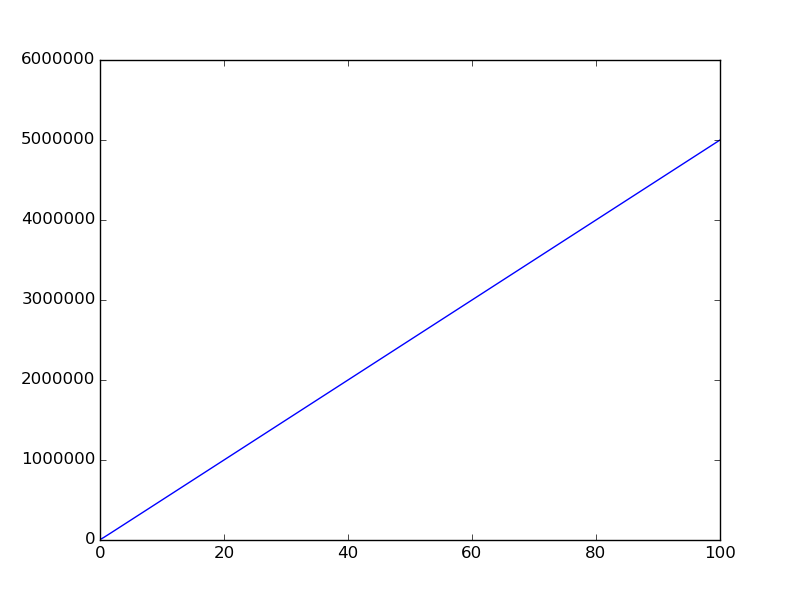
\includegraphics[width = \textwidth]{q2c_vel.png}
\end{figure}

In this condition, the electrical conductivity is expected to be constant as the equation is straight forward similar to the MHD equation and the value of n is assumed to be constant. 
\end{document}